%    Copyright (C)  2015  Fernando Pujaico Rivera. fernando.pujaico.rivera@gmail.com
%    Permission is granted to copy, distribute and/or modify this document
%    under the terms of the GNU Free Documentation License, Version 1.3
%    or any later version published by the Free Software Foundation;
%    with no Invariant Sections, no Front-Cover Texts, and no Back-Cover Texts.
%    A copy of the license is included with this file.
%
%
%    The last version of this template can be downloaded of http://trucomanx.github.io/BiospeckleData-Templates/
%
\documentclass[a4paper,10pt]{article}

\usepackage{graphicx}
\usepackage{caption}
\usepackage{subcaption}

\usepackage{hyperref}
\usepackage[bottom=2cm,top=3cm,left=3cm,right=2cm]{geometry}
\usepackage[utf8]{inputenc}
\usepackage[square,sort,comma,numbers]{natbib}
\bibliographystyle{unsrtnat}
\usepackage{listings}
\usepackage{color}
\definecolor{mygreen}{rgb}{0,0.6,0}
\definecolor{mygray}{rgb}{0.95,0.95,0.95}
\definecolor{mymauve}{rgb}{0.58,0,0.82}
\lstset{ %
  backgroundcolor=\color{mygray},   % choose the background color; you must add \usepackage{color} or \usepackage{xcolor}
  basicstyle=\footnotesize,        % the size of the fonts that are used for the code
  breaklines=true,                 % sets automatic line breaking
  commentstyle=\color{mygreen},    % comment style
  frame=single,	                   % adds a frame around the code
  keywordstyle=\color{blue},       % keyword style
  language=TeX,                    % the language of the code
  rulecolor=\color{black},         % if not set, the frame-color may be changed on line-breaks within not-black text (e.g. comments (green here))
}



% Title Page
\title{Biospeckle data of a maize seed}
\author{John Doe \\ \href{mailto:JohnDoe@deg.ufla.br}{JohnDoe@ufla.br} }

\begin{document}

\maketitle

\begin{abstract}
Images to research the development of a seeds viability test using the biospeckle technique.
\end{abstract}
~
\begin{minipage}[c]{0.5\textwidth}
\begin{tabular}{l |l}
\hline
\textbf{Name} 	& \textbf{Value}  \\ \hline \hline	
Biospeckle data	& Maize seed\\
Time rate	& 0.08 sec\\
Laser wavelength& 632.8 nm \\ 
Setup		& backscattering\\ 
\hline
Number of images& 100\\ 
Image format	& BMP 8bit grayscale \\
Size of images	& 490x256 pixels\\
\hline
First image	& 1.bmp\\ 
Last image	& 100.bmp\\ 
\hline
First reference of data	& \cite{ref1} \\ 
\hline
\end{tabular}
%\captionof{table}{Biospeckle data of a maize seed.}
\end{minipage}
\begin{minipage}[c]{0.5\textwidth}
\begin{center}
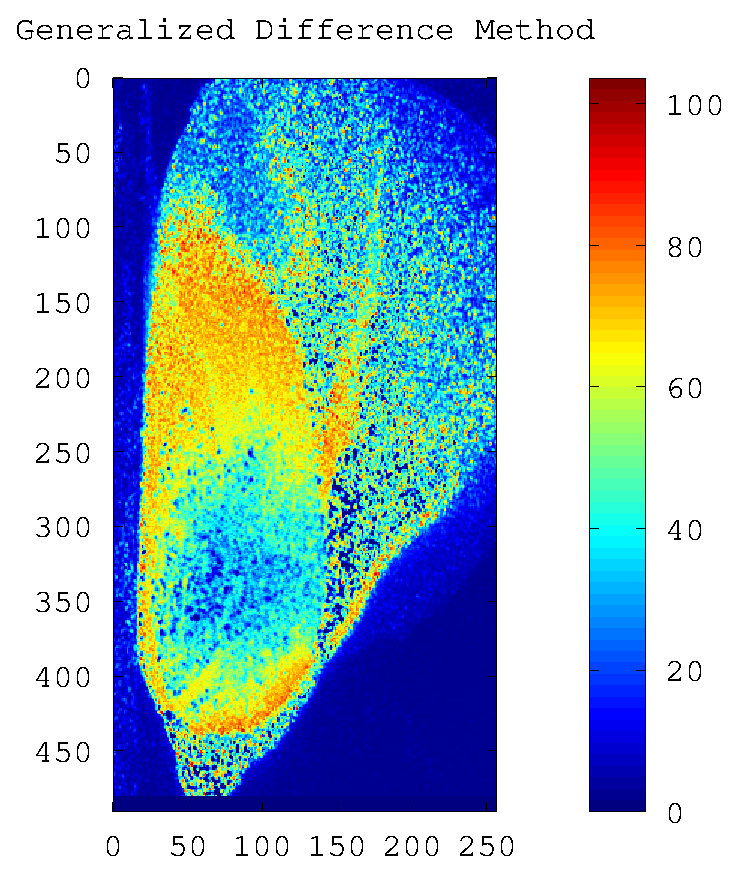
\includegraphics[width=0.6\linewidth]{example/testgendiff.eps}
\captionof{figure}{Example of biospeckle index.}
\end{center}
\end{minipage}


\section*{Details}
The images are located in the directory \lstinline!MaizeSeed!.

\section*{Citation}
We have invested a lot of time and effort in to get this data, please cite it
when using it \footnote{The template of this file report can be downloaded of 
\url{http://trucomanx.github.io/BiospeckleData-Templates/}}.
\begin{lstlisting}[language=Bash]
@misc{ maizeseed1,
    author = {John Doe},
    title  = {Biospeckle data of a maize seed},
    year   = {2015},
    url    = {http://repositorio.ufla.br/jspui/handle/1/10560},
 }
\end{lstlisting}


\begin{thebibliography}{9}
\bibitem{ref1}
John Doe and Jane Roe,
\emph{Study of biospeckle data},
Journal name, 2015.

\end{thebibliography}

\end{document}
   
